\documentclass[tikz,border=3pt]{standalone}
\usepackage[utf8]{inputenc}
\usepackage[T1]{fontenc}
\usepackage{lmodern}
\renewcommand{\familydefault}{\sfdefault}
\usepackage{amsmath}
\usepackage{sansmath}\sansmath
\usepackage{pgfplots}\pgfplotsset{compat=1.18,/pgf/number format/use comma,/pgf/number format/1000 sep={.}}
\usetikzlibrary{arrows.meta,calc,positioning,decorations.pathmorphing,patterns}
% paleta del sitio
\definecolor{nar}{HTML}{E8680C}\definecolor{narc}{HTML}{FFB35C}\definecolor{hielo}{HTML}{FFF3E8}
\definecolor{tinta}{HTML}{1D1D1F}\definecolor{gris}{HTML}{6E6E73}\definecolor{lila}{HTML}{7C5CF0}
\definecolor{azul}{HTML}{2F6FD6}\definecolor{menta}{HTML}{17A673}\definecolor{coral}{HTML}{E8342A}
\pgfplotsset{base/.style={axis lines=left,grid=major,grid style={gris!20},tick label style={font=\small},label style={font=\small},axis line style={tinta!80}}}
\begin{document}
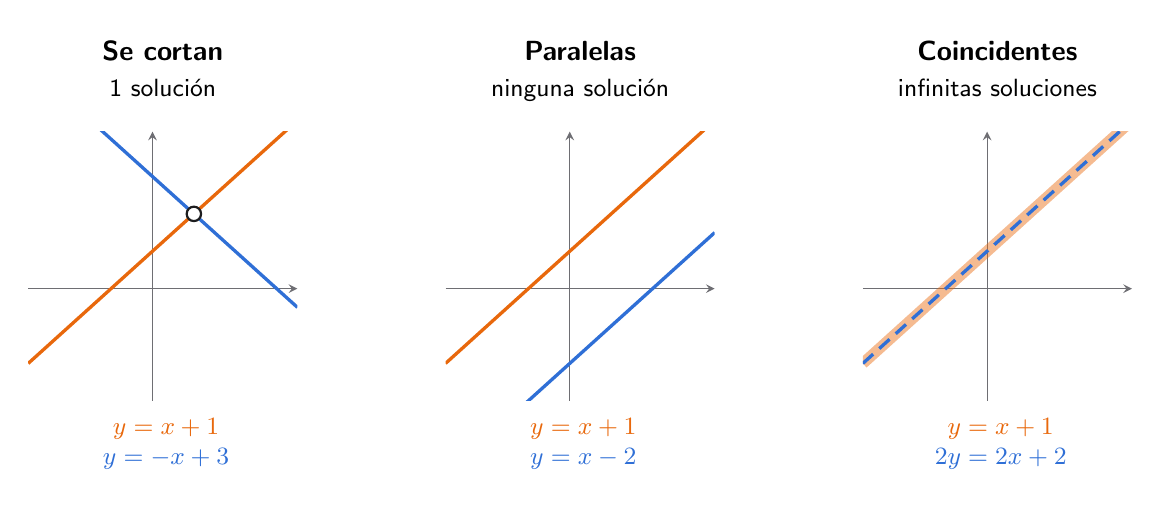
\begin{tikzpicture}
\begin{axis}[at={(0cm,0)},axis lines=middle,width=5cm,height=5cm,xmin=-3,xmax=3.5,ymin=-3,ymax=4.2,ticks=none,axis line style={gris},title={\textbf{\strut Se cortan}\\[1pt]{\small\strut 1 solución}},title style={align=center,font=\normalsize}]
\addplot[nar,very thick,domain=-3:3.5] {x+1};
\addplot[azul,very thick,domain=-3:3.5] {-x+3};
\addplot[only marks,mark=*,mark options={fill=white,draw=tinta,thick},mark size=2.6pt] coordinates {(1,2)};
\end{axis}
\node[align=center,font=\small,anchor=north] at ($(0cm,0)+(1.75cm,-0.1cm)$) {\textcolor{nar}{$y = x + 1$}\\\textcolor{azul}{$y = -x + 3$}};
\begin{axis}[at={(5.3cm,0)},axis lines=middle,width=5cm,height=5cm,xmin=-3,xmax=3.5,ymin=-3,ymax=4.2,ticks=none,axis line style={gris},title={\textbf{\strut Paralelas}\\[1pt]{\small\strut ninguna solución}},title style={align=center,font=\normalsize}]
\addplot[nar,very thick,domain=-3:3.5] {x+1};
\addplot[azul,very thick,domain=-3:3.5] {x-2};
\end{axis}
\node[align=center,font=\small,anchor=north] at ($(5.3cm,0)+(1.75cm,-0.1cm)$) {\textcolor{nar}{$y = x + 1$}\\\textcolor{azul}{$y = x - 2$}};
\begin{axis}[at={(10.6cm,0)},axis lines=middle,width=5cm,height=5cm,xmin=-3,xmax=3.5,ymin=-3,ymax=4.2,ticks=none,axis line style={gris},title={\textbf{\strut Coincidentes}\\[1pt]{\small\strut infinitas soluciones}},title style={align=center,font=\normalsize}]
\addplot[nar,line width=4pt,opacity=.45,domain=-3:3.5] {x+1};
\addplot[azul,very thick,dash pattern=on 5pt off 3pt,domain=-3:3.5] {x+1};
\end{axis}
\node[align=center,font=\small,anchor=north] at ($(10.6cm,0)+(1.75cm,-0.1cm)$) {\textcolor{nar}{$y = x + 1$}\\\textcolor{azul}{$2y = 2x + 2$}};
\end{tikzpicture}
\end{document}
